\documentclass{assignment}
\ProjectInfos{光电子技术}{PHYS6651P}{2021-2022学年第一学期}{第五章作业}{}{陈稼霖}[https://github.com/Chen-Jialin]{SA21038052}

\begin{document}
\begin{prob}
    已知一阶跃光纤芯区和包层折射率分别为 $n_1=1.62$,$n_2=1.52$.
    \begin{itemize}
        \item[(a)] 试计算光纤的数值孔径 NA$=$?
        \item[(b)] 计算空气中该光线的最大入射角 $\theta_M=$?
        \item[(c)] 如果将光纤浸入水中($n_{\text{水}}=1.33$),$\theta_M=$?
    \end{itemize}
\end{prob}
\begin{sol}
    \begin{itemize}
        \item[(a)] 该光纤的数值孔径为
        \begin{align}
            \text{NA}=\sqrt{n_1^2-n_2^2}=0.560
        \end{align}
        \item[(b)] 空气中该光纤的最大入射角为
        \begin{align}
            \theta_M=\arcsin\text{NA}=0.595(\text{rad})=34.1^{\circ}.
        \end{align}
        \item[(c)] 如果将光纤浸入水中,则其数值孔径为
        \begin{align}
            \text{NA}=\frac{1}{n_{\text{水}}}\sqrt{n_1^2-n_2^2},
        \end{align}
        最大入射角为
        \begin{align}
            \theta_M=\arcsin\text{NA}=\arcsin\left(\frac{1}{n_{\text{水}}}\sqrt{n_1^2-n_2^2}\right)=0.435(\text{rad})=24.9^{\circ}.
        \end{align}
    \end{itemize}
\end{sol}

\begin{prob}
    设阶跃光纤的数值孔径 NA$=0.2$,芯(半)径 $a=60\,\mu$m,$\lambda_0=0.9\,\mu$m,计算光纤传输的总模数.
\end{prob}
\begin{sol}
    该阶跃光纤的归一化频率为
    \begin{align}
        V=\frac{\omega a}{c}\sqrt{n_1^2-n_2^2}=\frac{2\pi a}{\lambda}\sqrt{n_1^2-n_2^2}=\frac{2\pi a}{\lambda}\text{NA}=83.78
    \end{align}
    故该光纤传输的总模数约为
    \begin{align}
        \frac{V^2}{2}=3509.
    \end{align}
\end{sol}

\begin{prob}
    欲设计阶跃单模光纤,其芯折射率为 $n_1=1.5$,$\Delta=0.005$,试分别计算波长为 $\lambda_0=1.3\,\mu$m 和 $\lambda_0=0.6328\,\mu$m 的最大芯(半)径.
\end{prob}
\begin{sol}
    要使光纤仅支持单模, 则支持的模式应为没有截止频率的 $HE_{11}$ 模, 且光纤的工作频率应低于截止频率最低的 $TE_{01}$ (或 $TM_{01}$) 模, 即:
    \begin{gather}
        \omega=\frac{2\pi c}{\lambda_0}\leq\frac{2.405c}{a\sqrt{n_1^2-n_2^2}}=\frac{2.405c}{an_1\sqrt{2\Delta}}\\
        \Longrightarrow a\leq\frac{2.405\lambda_0}{2\pi n_1\sqrt{2\Delta}}.
    \end{gather}
    故对 $\lambda_0=1.3\,\mu$m, 最大纤芯为 $3.32\,\mu$m; 对 $\lambda_0=0.6328\,\mu$m, 最大纤芯为 $1.61\,\mu$m.
\end{sol}

\begin{prob}
    设一根光纤的芯的折射率 $n_1=1.532$,包层的折射率 $n_2=1.530$
    \begin{itemize}
        \item[(a)] 计算临界角;
        \item[(b)] 设一条光线沿轴向传播,另一条光线以临界角射到包层上,试求轴向光线传播 $1$ 公里后两光线的滞后.
    \end{itemize}
\end{prob}
\begin{sol}
    \begin{itemize}
        \item[(a)] 临界角为
        \begin{align}
            \varphi=\arcsin\frac{n_2}{n_1}=1.52(\text{rad})=87.1^{\circ}.
        \end{align}
        \item[(b)] 轴向光线传播 $1$ 公里后两光线的滞后距离为
        \begin{align}
            \Delta l=1\text{ km}\times(1-\sin\varphi)=1\text{ km}\times\left(1-\frac{n_2}{n_1}\right)=1.31\times 10^{-3}\text{ km}=1.31\text{ m},
        \end{align}
        滞后时间为
        \begin{align}
            \Delta t=\frac{\Delta l}{c/n_1}=6.67\times 10^{-9}\text{ s}=6.67\text{ s}.
        \end{align}
    \end{itemize}
\end{sol}

\begin{prob}
    已知一直圆柱形阶跃光纤,纤芯和包层折射率分别为 $n_1=1.62$,$n_2=1.52$,其纤芯直径 $d=10\,\mu$m,弯曲后的曲率半径 $R=1.0$ cm.
    \begin{itemize}
        \item[(a)] 试计算放在空气中子午光线的最大入射角 $\theta_M$?
        \item[(b)] $R$ 值低于多少时,子午光线便不在内表面上反射?(入射角 $\theta_0=\theta_M$)(只要有一条子午光线做到就可以)
        \item[(c)] 对该光纤,要使最大孔径角 $\theta_M$ 增大到 $90^{\circ}$,则 $n_2$ 最大应等于多少?(设纤芯的折射率保持一定.)
        \item[(d)] 当 $\theta_M=90^{\circ}$ 时,出射光会不会在光纤的出射端面上发生全反射?(试分析之)
    \end{itemize}
\end{prob}
\begin{sol}
    \begin{itemize}
        \item[(a)] 放在空气中子午光线的最大入射角为
        \begin{align}
            \theta_M=\arcsin\left[n_1^2-\left(\frac{R+d/2}{R-d/2}\right)^2n_2^2\right]^{1/2}=0.590(\text{rad})=33.8^{\circ}.
        \end{align}
        \item[(b)] 当以 $\theta_M$ 入射角入射,子午光线在光纤直部的纤芯-包层分界面上的反射角 $\varphi_0$ 满足
        \begin{align}
            \cos\varphi_0=\frac{1}{n_1}\sin\theta_M=0.343,
        \end{align}
        光线在光纤弯部内侧的纤芯-包层分界面上的反射角为
        \begin{align}
            \sin\varphi_2=\frac{R+x}{R-d/2}\sin\varphi_0=\frac{R+x}{R-d/2}\sqrt{1-\cos^2\varphi_0},
        \end{align}
        其中 $x$ 为光线由光纤直部进入弯部处与子午线的距离,$-d/2\leq x\leq d/2$. 当
        \begin{align}
            \sin\varphi_2=1\Longrightarrow R=\frac{x\sqrt{1-\cos^2\varphi_0}+d/2}{1-\sqrt{1-\cos^2\varphi_0}}
        \end{align}
        时,光线恰好与内表面相切而不反射,即当
        \begin{align}
            R\leq 1.60\times 10^{-4}\text{ m}=160\,\mu\text{m}
        \end{align}
        时,($x=d/2$ 的)子午光线便不在内表面上反射.
        \item[(c)] 要使最大孔径角 $\theta_M$ 增大到 $90^{\circ}$,
        \begin{align}
            \sin\theta_M=\left[n_1^2-\left(\frac{R+d/2}{R-d/2}\right)^2n_2^2\right]^{1/2}=1,
        \end{align}
        即 $n_2$ 最大应为
        \begin{align}
            n_2=1.27
        \end{align}
        \item[(d)] 根据弯曲光纤的对称性和光路的可逆性,光线在出射端面上的出射角应当与其在入射端面上的入射角相等。故当 $\theta_M=90^{\circ}$ 时,出射光\uline{不会}在光纤的出射端面上发生全反射.
    \end{itemize}
\end{sol}

\begin{prob}
    已知一圆柱形阶跃光纤的出射端面有 $\alpha=10^{\circ}$ 倾角,纤芯和包层折射率分别为 $n_1=1.62$,$n_2=1.52$,出射端面仍垂直于轴线(不考虑光纤弯曲)
    \begin{itemize}
        \item[(a)] 试计算放在空气中光纤的最大入射角 $\theta_{\max}$.
        \item[(b)] 要使 $\theta_{\max}=90^{\circ}$,该光纤的数值孔径 NA 至少要多少?这一光线($\theta_M=90^{\circ}$)会不会在出射端面发生全反射?(设包层折射率一定)
    \end{itemize}
\end{prob}
\begin{sol}
    \begin{itemize}
        \item[(a)] 当光线以如图 \ref{1-6-1} 的角度从空气入射,则光纤的最大入射角为
        \begin{align}
            \theta_{\max}=\arcsin\left(\sqrt{n_1^2-n_2^2}\cos\alpha-n_2\sin\alpha\right)=0.292(\text{rad})=16.7^{\circ}.
        \end{align}
        \begin{figure}[h]
            \centering
            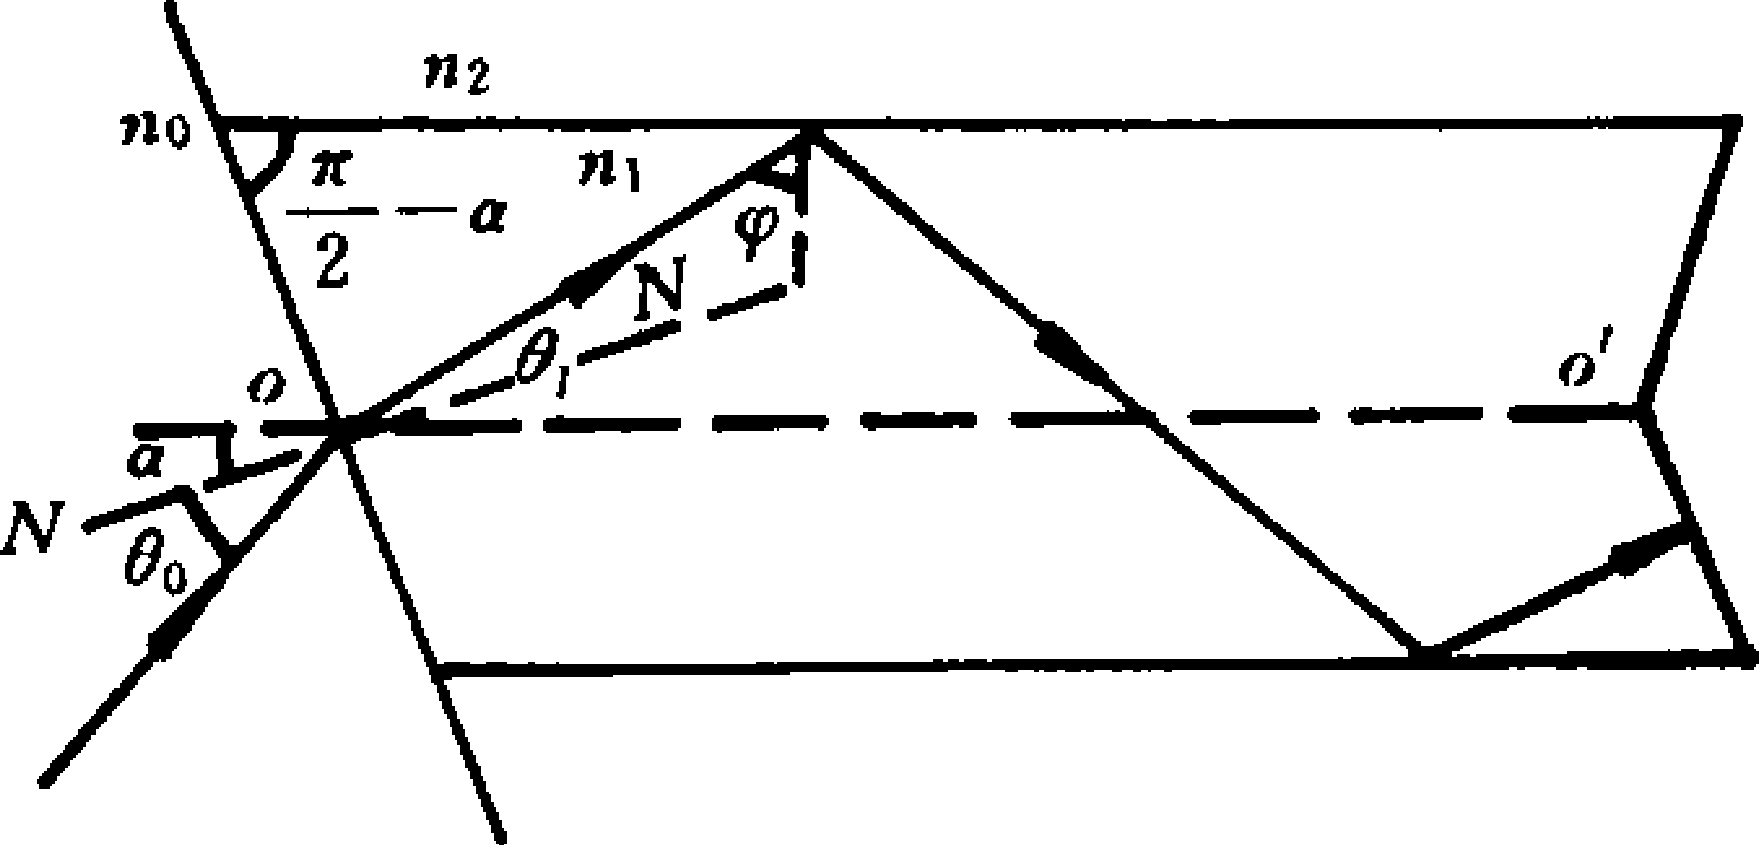
\includegraphics[width=.5\columnwidth]{1-5-1.png}
            \caption{}
            \label{1-6-1}
        \end{figure}

        当光线从法线另一侧入射,如图 \ref{1-6-2},则光纤的最大入射角为
        \begin{align}
            \theta_{\max}=\arcsin\left(\sqrt{n_1^2-n_2^2}\cos\alpha+n_2\sin\alpha\right)=0.95(\text{rad})=54.7^{\circ}.
        \end{align}
        \begin{figure}[h]
            \centering
            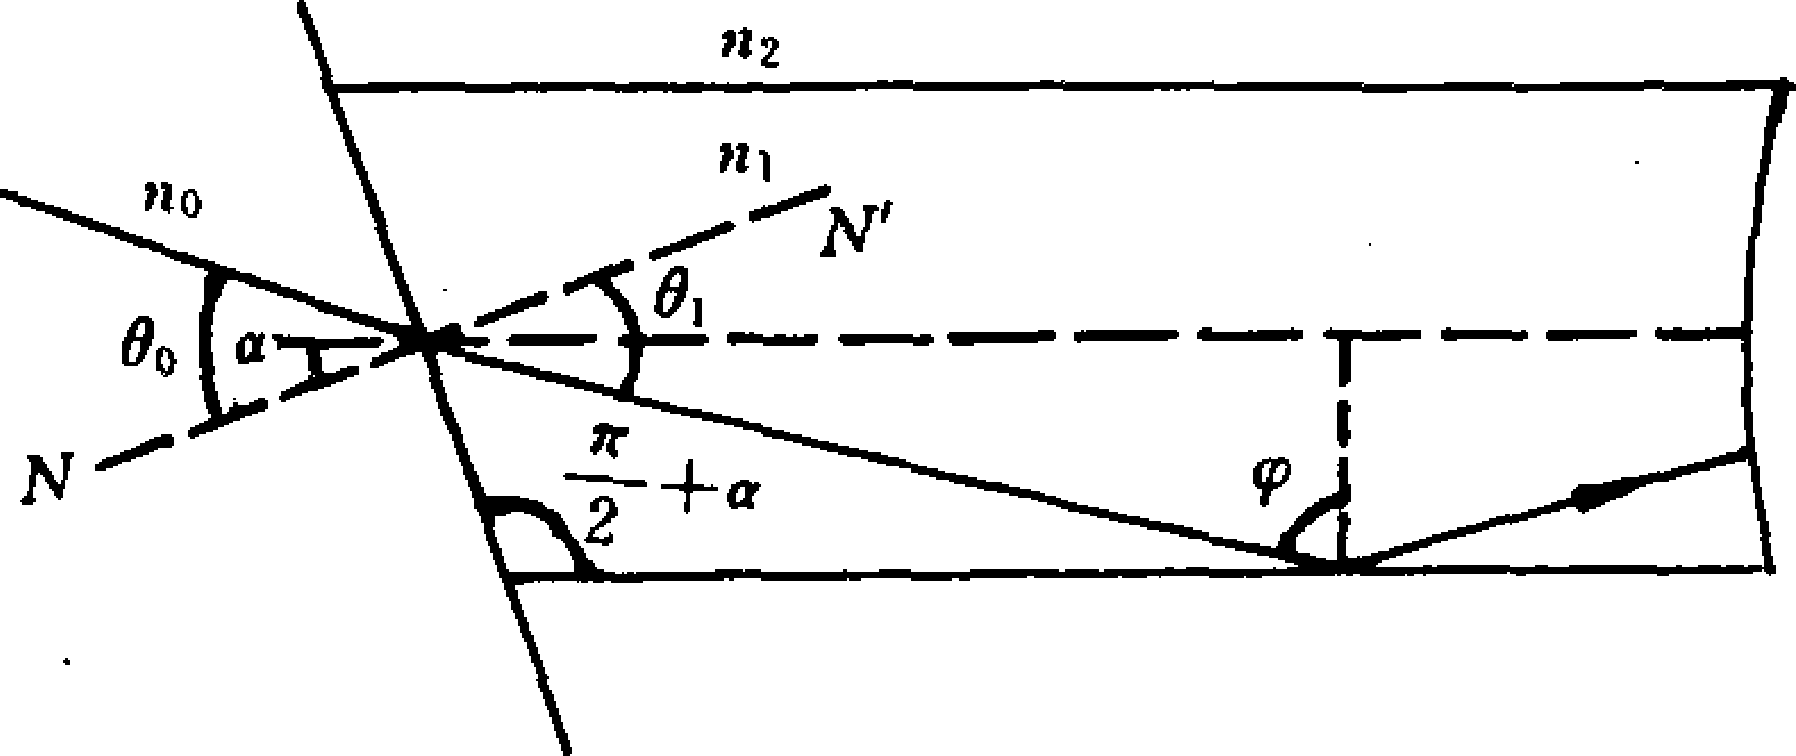
\includegraphics[width=.5\columnwidth]{1-5-2.png}
            \caption{}
            \label{1-6-2}
        \end{figure}
        \item[(b)] 对于图 \ref{1-6-1} 所示的情况,要使 $\theta_{\max}=90^{\circ}$,该光纤的数值孔径至少为
        \begin{align}
            \text{NA}=\frac{1+n_2\sin\alpha}{\cos\alpha}=1.54
        \end{align}
        此时,这一光线($\theta_M=90^{\circ}$)在纤芯-包层交界面上的反射角 $\varphi$ 满足
        \begin{align}
            \sin\varphi=\frac{n_2}{n_1}.
        \end{align}
        因为在出射端面上
        \begin{align}
            n_1\cos\varphi=n_1\sqrt{1-\left(\frac{n_2}{n_1}\right)^2}=\text{NA}>1,
        \end{align}
        所以这一光线\uline{会}在出射端面上发生全反射.

        对于图 \ref{1-6-2} 所示的情况,要使 $\theta_{\max}=90^{\circ}$,该光纤的数值孔径至少为
        \begin{align}
            \text{NA}=\frac{1-n_2\sin\alpha}{\cos\alpha}=0.747
        \end{align}
        因为在出射端面上
        \begin{align}
            n_1\cos\varphi=\text{NA}<1,
        \end{align}
        所以这一光线\uline{不会}在出射端面上发生全反射.
    \end{itemize}
\end{sol}
\end{document}